\chapter{The Cosmic Microwave Backgound}

\section{The Expanding Universe and the \texorpdfstring{$\Lambda$}{LAMBDA-}CDM Model}
\subsection{The Hubble's Law}\label{ss:hubbleslaw}

In 1929, Edwin Hubble examined the relationship between the distances of
some galaxies and their radial velocities, inferred from their \emph{redshifts},
and formulated an empirical law, which states direct proportionality
between these two quantities (\autoref{fig:hubbleslaw}):

\begin{equation}\label{eq:hubble_law}
        \vb{v} = H_0 \vb{d}
\end{equation}

where $H_0$ is the \emph{Hubble constant}.

\begin{figure}
        \centering
        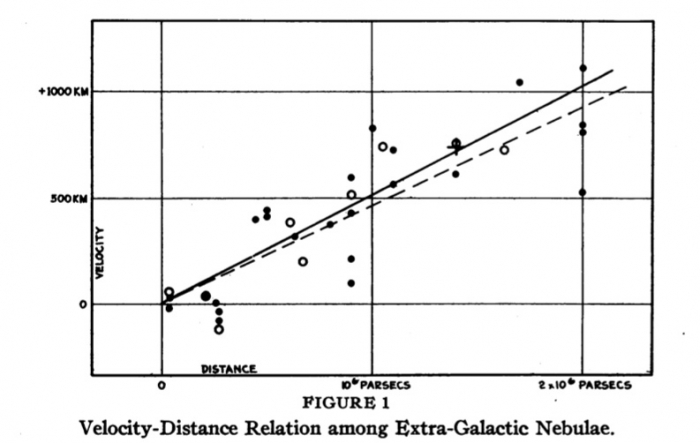
\includegraphics[width=\textwidth]{hubbleslaw}
        \caption{Hubbles Law}
        \label{fig:hubbleslaw}
\end{figure}

The observed \emph{redshifts} couldn't be explained by the proper motion of
the galaxies, instead this phenomenon was caused by the continuos expansion
of our universe.

An expanding universe was first theorized by Friedmann in 1922, before Hubble's
observations, as a consequence of the field equations of the theory of the
\emph{General Relativity} (GR). The starting point of Friedmann derivation was
an elegant and powerful assumption about the structure of our universe:
the \emph{Cosmological Principle}.

\section{The CMB Radiation}

\begin{figure}
        \centering
        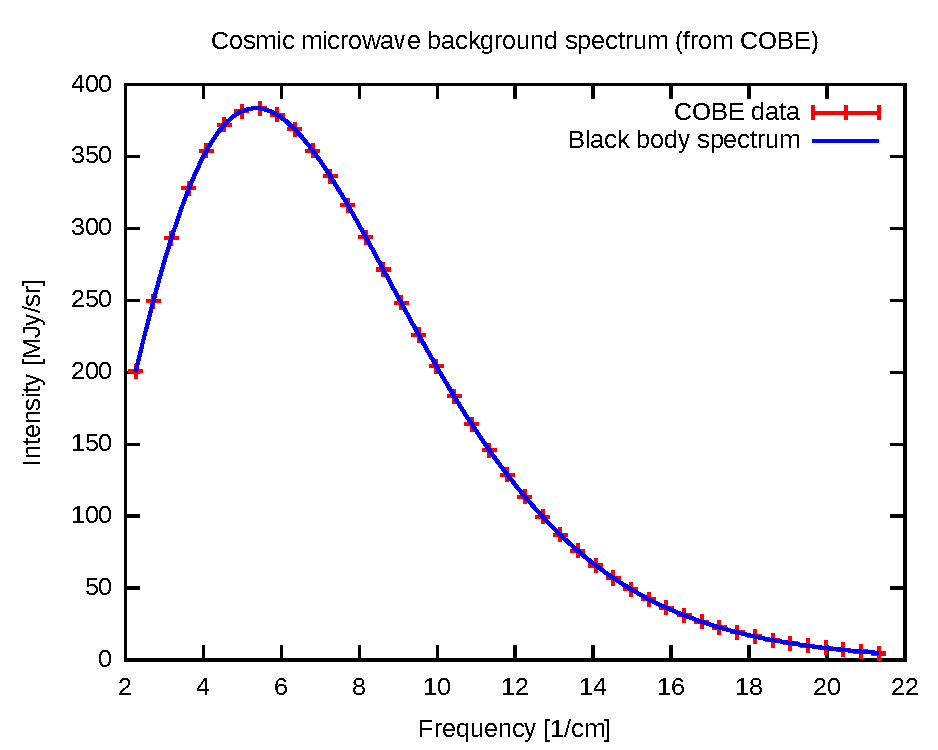
\includegraphics[width=\textwidth]{CMB_Spectrum_COBE}
        \caption{CMB Spectrum COBE}
        \label{fig:cmb_spectrum_cobe}
\end{figure}

\section{The CMB Temperature Anisotropies}

\begin{figure}
        \centering
        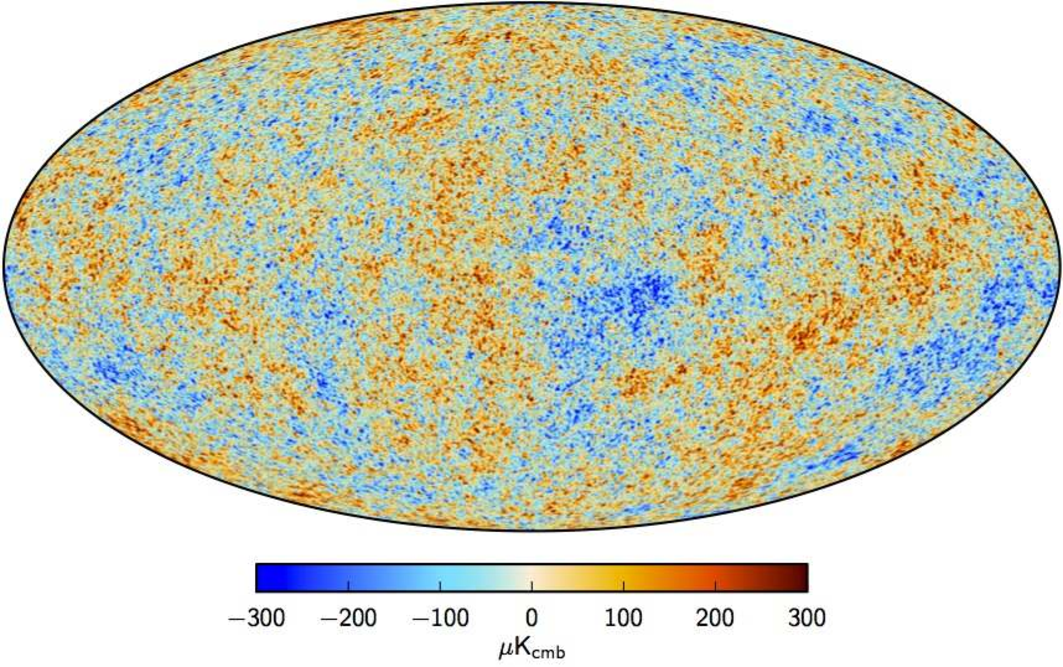
\includegraphics[width=\textwidth]{Planck_CMB}
        \caption{CMB Anisotropies Planck}
        \label{fig:plack_cmb}
\end{figure}

\section{The CMB Polarization}
